\chapter{Code}

%\chapter{Sources}
%\label{ch:sources}
%
%\begin{landscape}
%\begin{longtable}{cccccccc} \toprule
%\tableheadline{Source}&\tableheadline{4U}&\tableheadline{GX}&\tableheadline{IGR}&\tableheadline{INTEGRAL1}&\tableheadline{SWIFT}&\tableheadline{X}&\tableheadline{XTE}\\
%\midrule
%\endhead
%4U 0614+09&0614+091& & &4&J0617.1+0908& & \\
%4U 1636-53&1636-5& & &30&J1640.9-5345& & \\
%4U 1702-43&1702-42&340-00& &4&J1706.2-4302&Ara X-1& \\
%4U 1705-44&1705-440& & &43&J1708.8-4406& & \\
%4U 1728-34&1728-33&354+00& &58&J1731.9-3349& & \\
%Aql X-1&1908+00& & & &J1911.2+0034&Aql X-1& \\
%Cir X-1&1516-56& & &4&J1520.6-5710&Cir X-1& \\
%Cyg X-2&2142+38& & &22&J2144.6+3819&Cyg X-2& \\
%EXO 0748-676& & & & &J0748.5-6742& & \\
%GX 17+2&1813-1&17+01& &87&J1816.0-1402&Ser X-2& \\
%%GX 3+1&1744-26&3+01& &73&J1747.9-2633&Sgr X-1& \\
%GX 340+0&1642-45&340+00& &32&J1645.8-4536& & \\
%GX 349+2&1702-36&349+02& &40&J1705.7-3625&Sco X-2& \\
%GX 5-1&1758-25&5-01& &78&J1801.1-2504& & \\
%HETE J1900.1-2455& & & & &J1900.1-2453& & \\
%IGR J00291+5934& & &J00291+5934& & & & \\
%IGR J17480-2446& & &J17480-2446& & & & \\
%IGR J17498-2921& & &J17498-2921& & & & \\
%KS 1731-260& & & & & & & \\
%SAX J1808.4-3658& & & & &J1808.5-3655& &J1808-369\\
%SWIFT J1756.9-2508& & & & &J1756.9-2508& & \\
%Sco X-1&1617-15& & &2&J1620.1-1539&Sco X-1& \\
%Sgr X-1&1744-26&3+01& &73&J1747.9-2633&Sgr X-1& \\
%Sgr X-2&1811-17&13.5& &85&J1814.5-1708&Sgr X-2& \\
%V4634 Sgr&1826-2& & &92&J1829.5-2347& & \\
%XB 1254-690&1254-69& & & &J1257.4-6915& & \\
%XTE J0929-314& & & & & & &J0929-314\\
%XTE J1701-462& & & & &J1700.9-4611& &J1701-462\\
%XTE J1751-305& & & & & & &J1751-305\\
%XTE J1807-294& & & &83& & &J1807-294\\
%XTE J1814-338& & & & & & &J1814-338\\
%\midrule
%GX 339-4&1659-48&339-04& &38&J1702.8-4847& & \\
%H1743-322& & &J17464-3213&68&J1746.2-3213& &J1746-322\\
%XTE J1550-564& & & &7& & &J1550-564\\
%\bottomrule
%\caption[Alternative source names]{Overview of various alternative sources names as classified by \citet{SIMBAD}, grouped into neutron stars (above the horizontal line) and black holes (below the horizontal line). The leftmost column gives the source names used throughout this work.}\label{tab:aka}
%\end{longtable}
%\end{landscape}
%
%\chapter{Power Spectra}
%\label{ch:psds}
%\begin{figure}[p]
%	\myfloatalign
%	{\vspace*{-0.5cm}\hspace*{-1.5cm}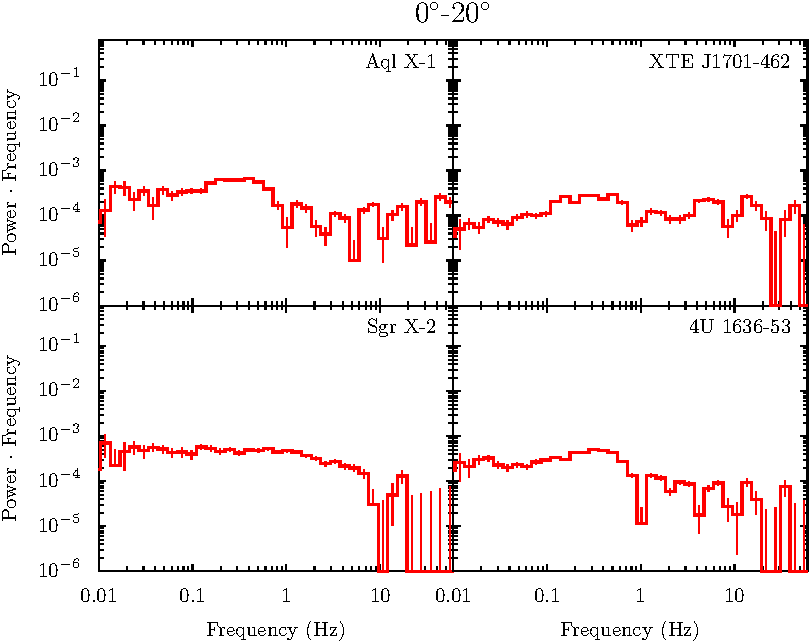
\includegraphics[width=1.13\linewidth]{ps/0_20}}
%	\caption[Power spectra with a hue of 0$^\circ$--20$^\circ$]{Representative power spectra within a hue range of 0$^\circ$--20$^\circ$}\label{fig:ps_0_20}
%\end{figure}
%\captionsetup[figure]{list=no}
%\begin{figure}[p]
%	\myfloatalign
%	{\vspace*{-0.5cm}\hspace*{-1.5cm}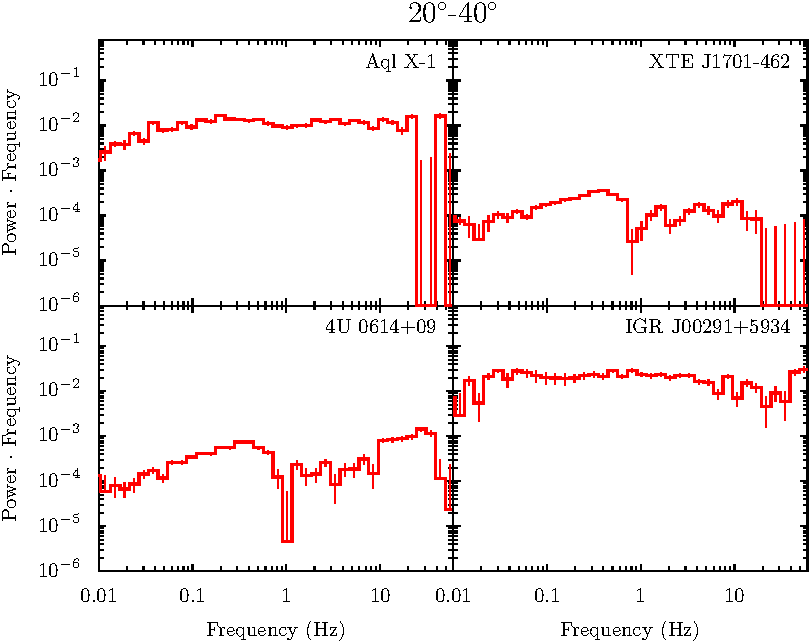
\includegraphics[width=1.13\linewidth]{ps/20_40}}
%	\caption[Power spectra with a hue of 20$^\circ$--40$^\circ$]{Representative power spectra within a hue range of 20$^\circ$--40$^\circ$}\label{fig:ps_20_40}
%\end{figure}
%
%\begin{figure}[p]
%	%\myfloatalign
%	{\vspace*{-0.5cm}\hspace*{-1.5cm}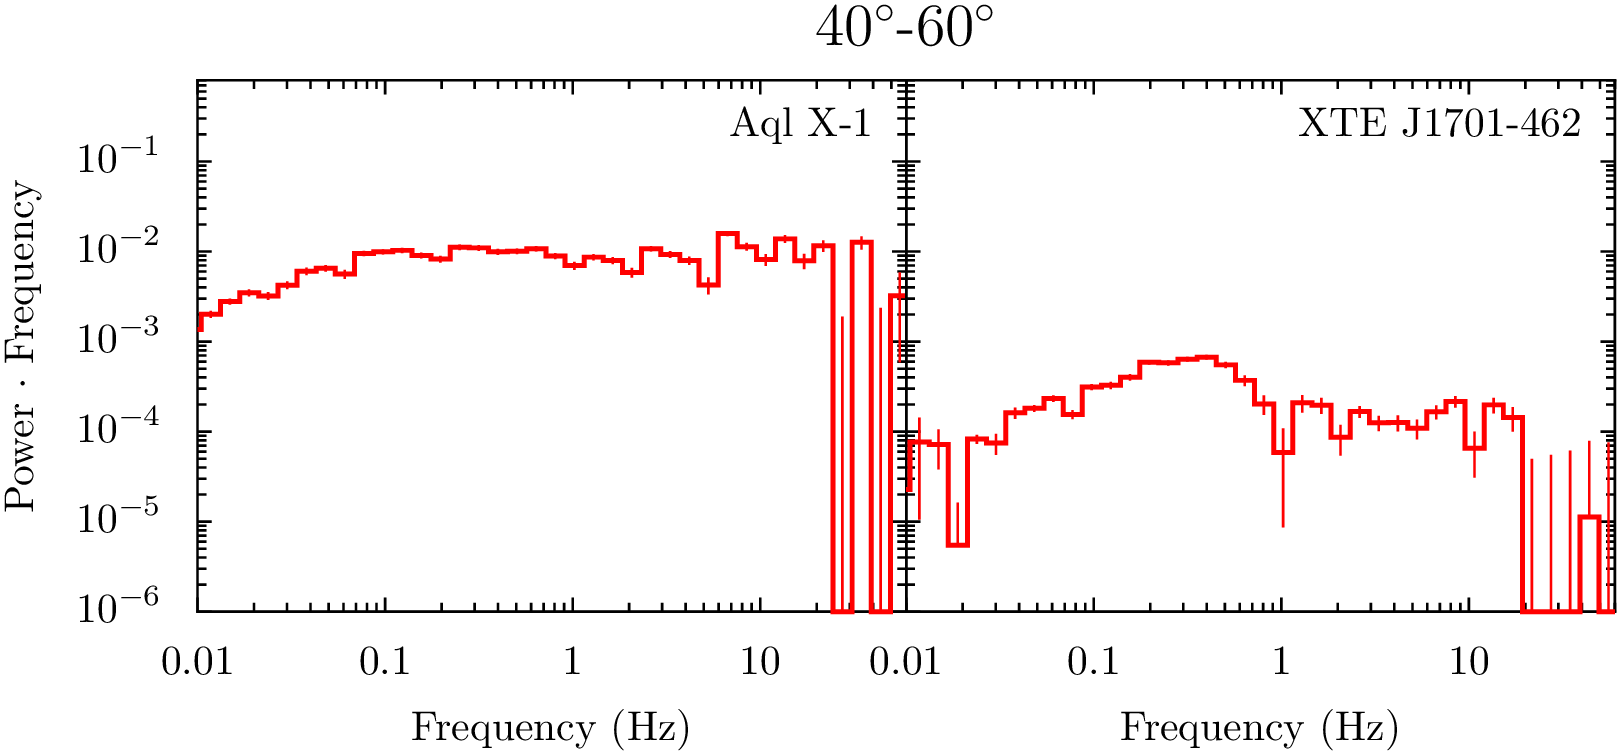
\includegraphics[width=1.13\linewidth]{ps/40_60}}
%	\caption[Power spectra with a hue of 40$^\circ$--60$^\circ$]{Representative power spectra within a hue range of 40$^\circ$--60$^\circ$}\label{fig:ps_40_60}
%\end{figure}
%
%\begin{figure}[p]
%	%\myfloatalign
%	{\vspace*{-0.5cm}\hspace*{-1.5cm}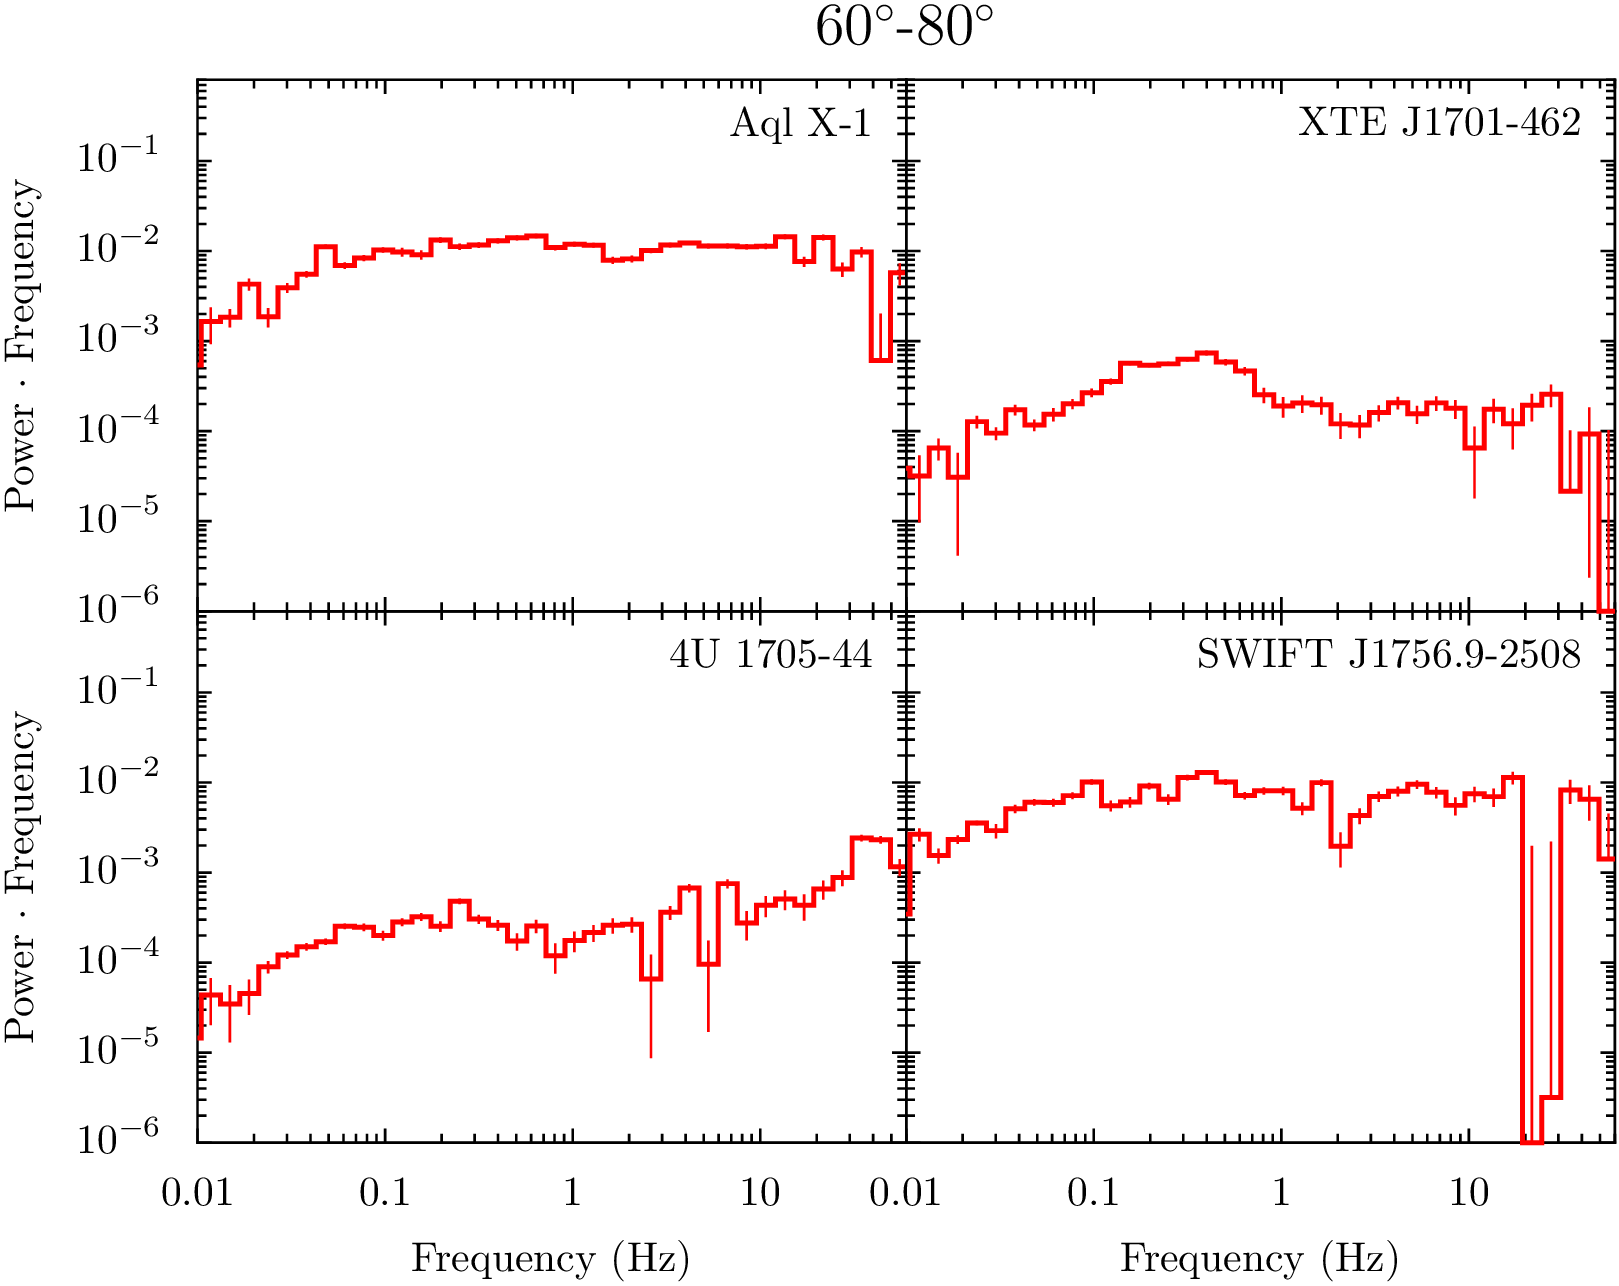
\includegraphics[width=1.13\linewidth]{ps/60_80}}
%	\caption[Power spectra with a hue of 60$^\circ$--80$^\circ$]{Representative power spectra within a hue range of 60$^\circ$--80$^\circ$}\label{fig:ps_60_80}
%\end{figure}
%
%\begin{figure}[p]
%	%\myfloatalign
%	{\vspace*{-0.5cm}\hspace*{-1.5cm}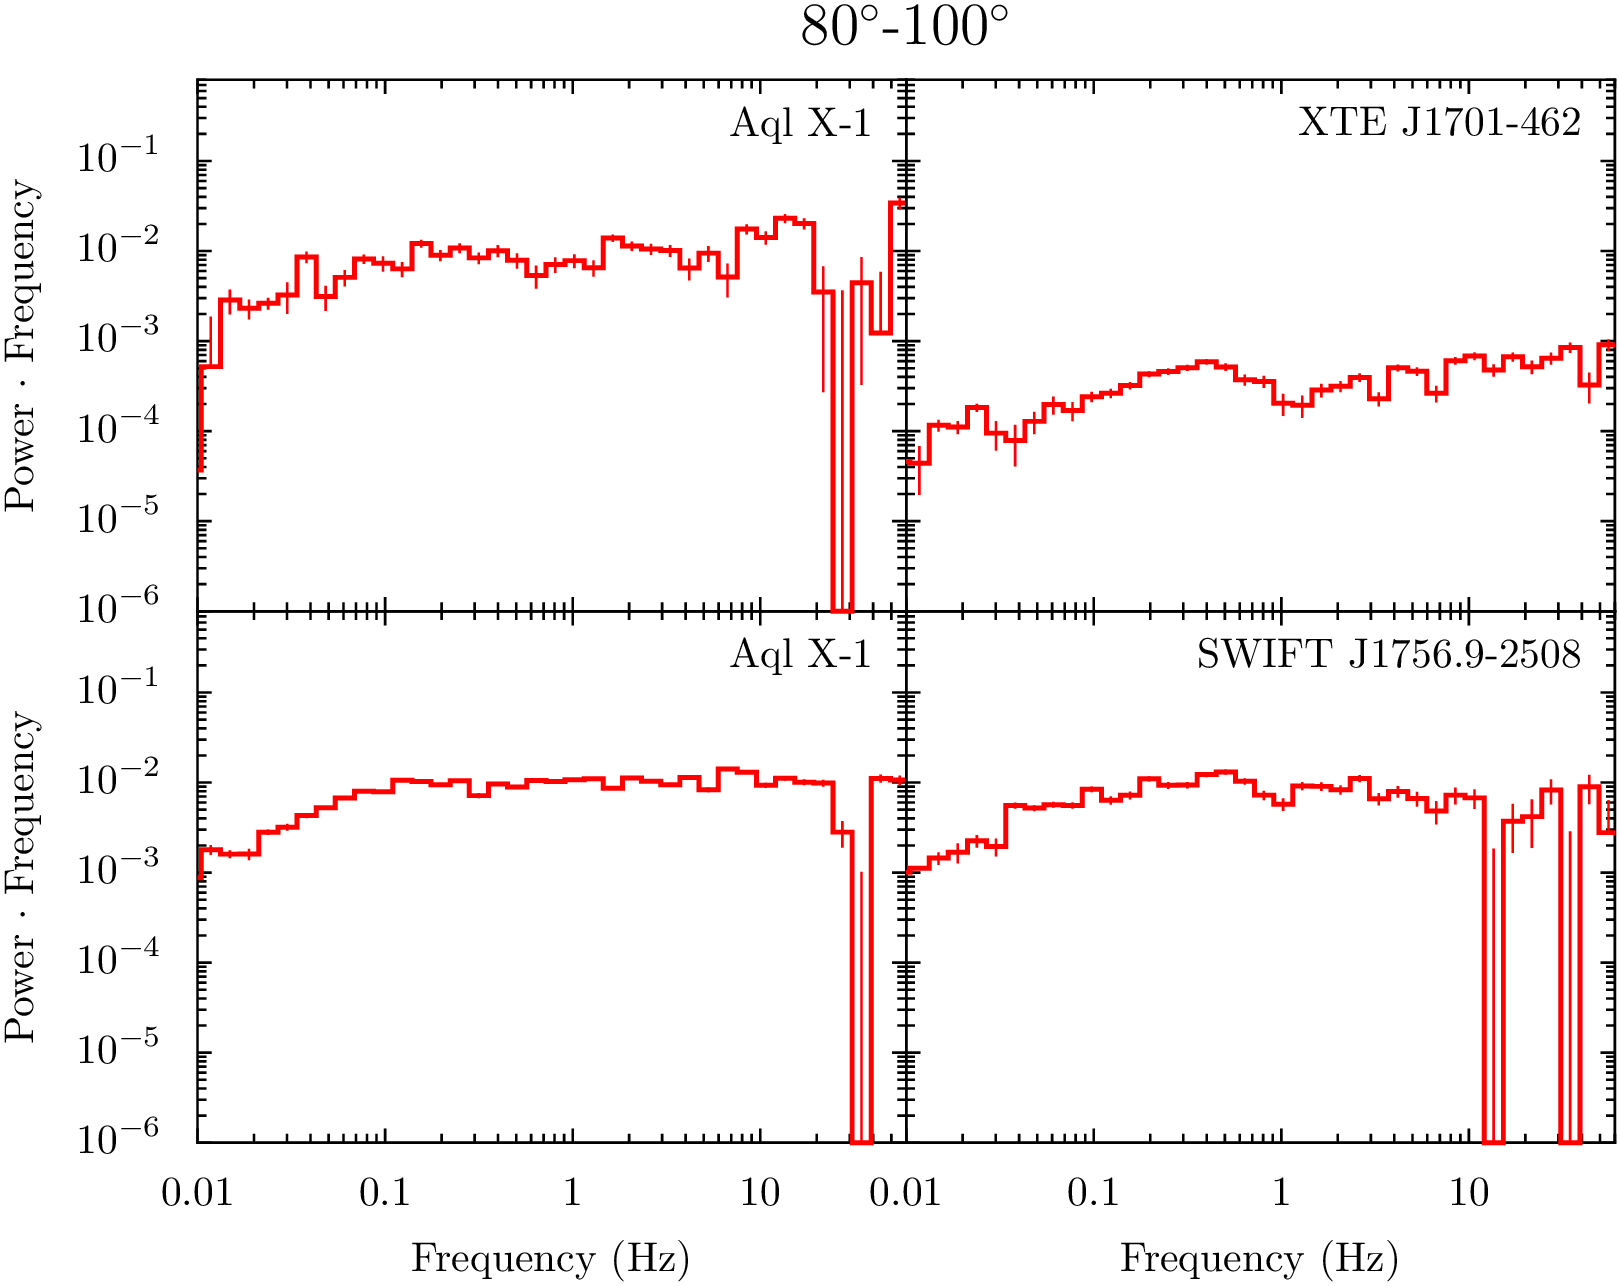
\includegraphics[width=1.13\linewidth]{ps/80_100}}
%	\caption[Power spectra with a hue of 80$^\circ$--100$^\circ$]{Representative power spectra within a hue range of 80$^\circ$--100$^\circ$}\label{fig:ps_80_100}
%\end{figure}
%
%\begin{figure}[p]
%	%\myfloatalign
%	{\vspace*{-0.5cm}\hspace*{-1.5cm}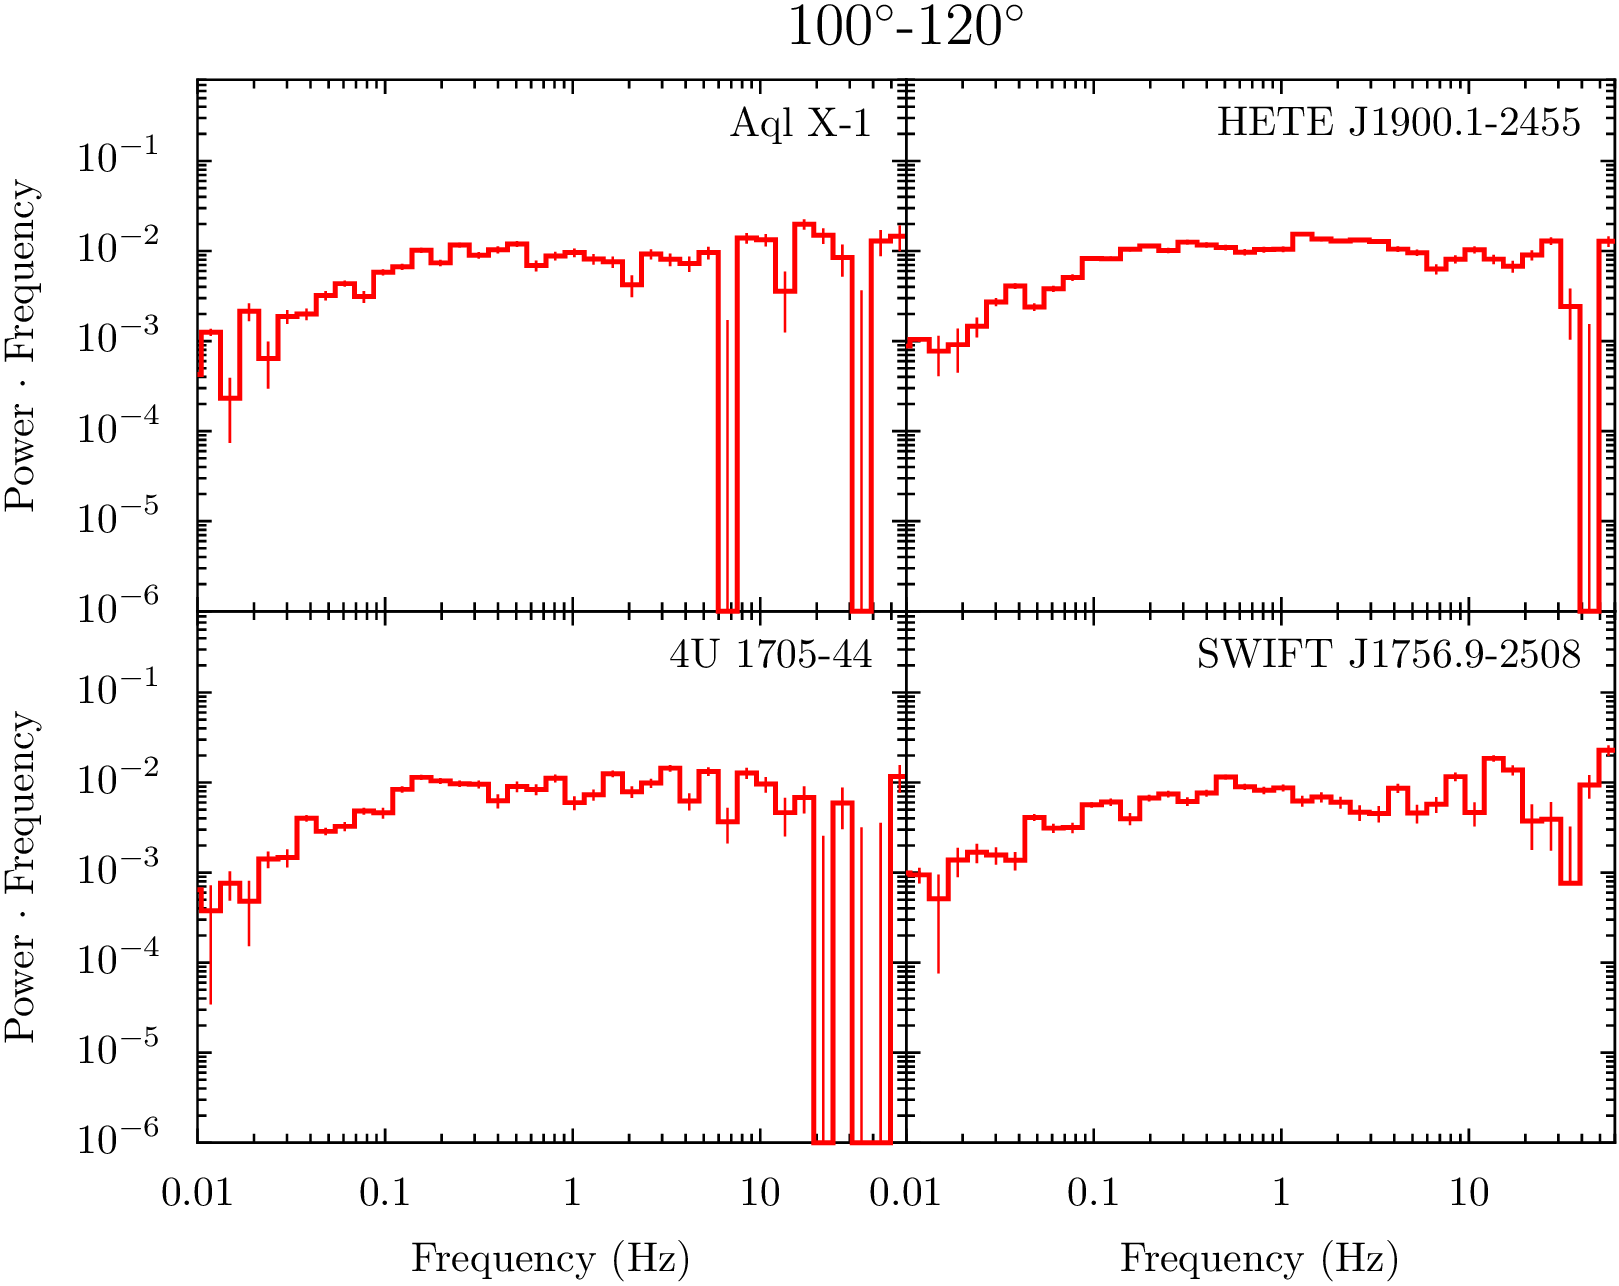
\includegraphics[width=1.13\linewidth]{ps/100_120}}
%	\caption[Power spectra with a hue of 100$^\circ$--120$^\circ$]{Representative power spectra within a hue range of 100$^\circ$--120$^\circ$}\label{fig:ps_100_120}
%\end{figure}
%
%\begin{figure}[p]
%	%\myfloatalign
%	{\vspace*{-0.5cm}\hspace*{-1.5cm}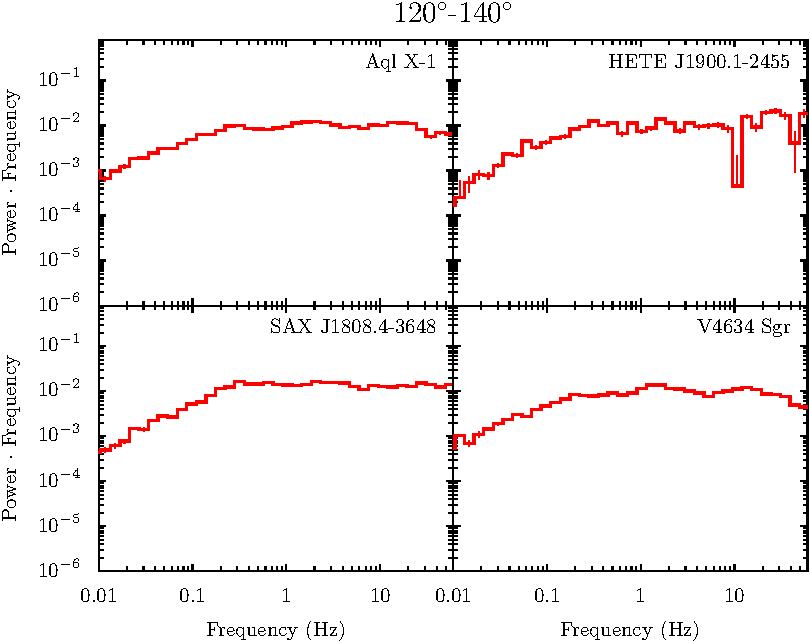
\includegraphics[width=1.13\linewidth]{ps/120_140}}
%	\caption[Power spectra with a hue of 120$^\circ$--140$^\circ$]{Representative power spectra within a hue range of 120$^\circ$--140$^\circ$}\label{fig:ps_120_140}
%\end{figure}
%
%\begin{figure}[p]
%	%\myfloatalign
%	{\vspace*{-0.5cm}\hspace*{-1.5cm}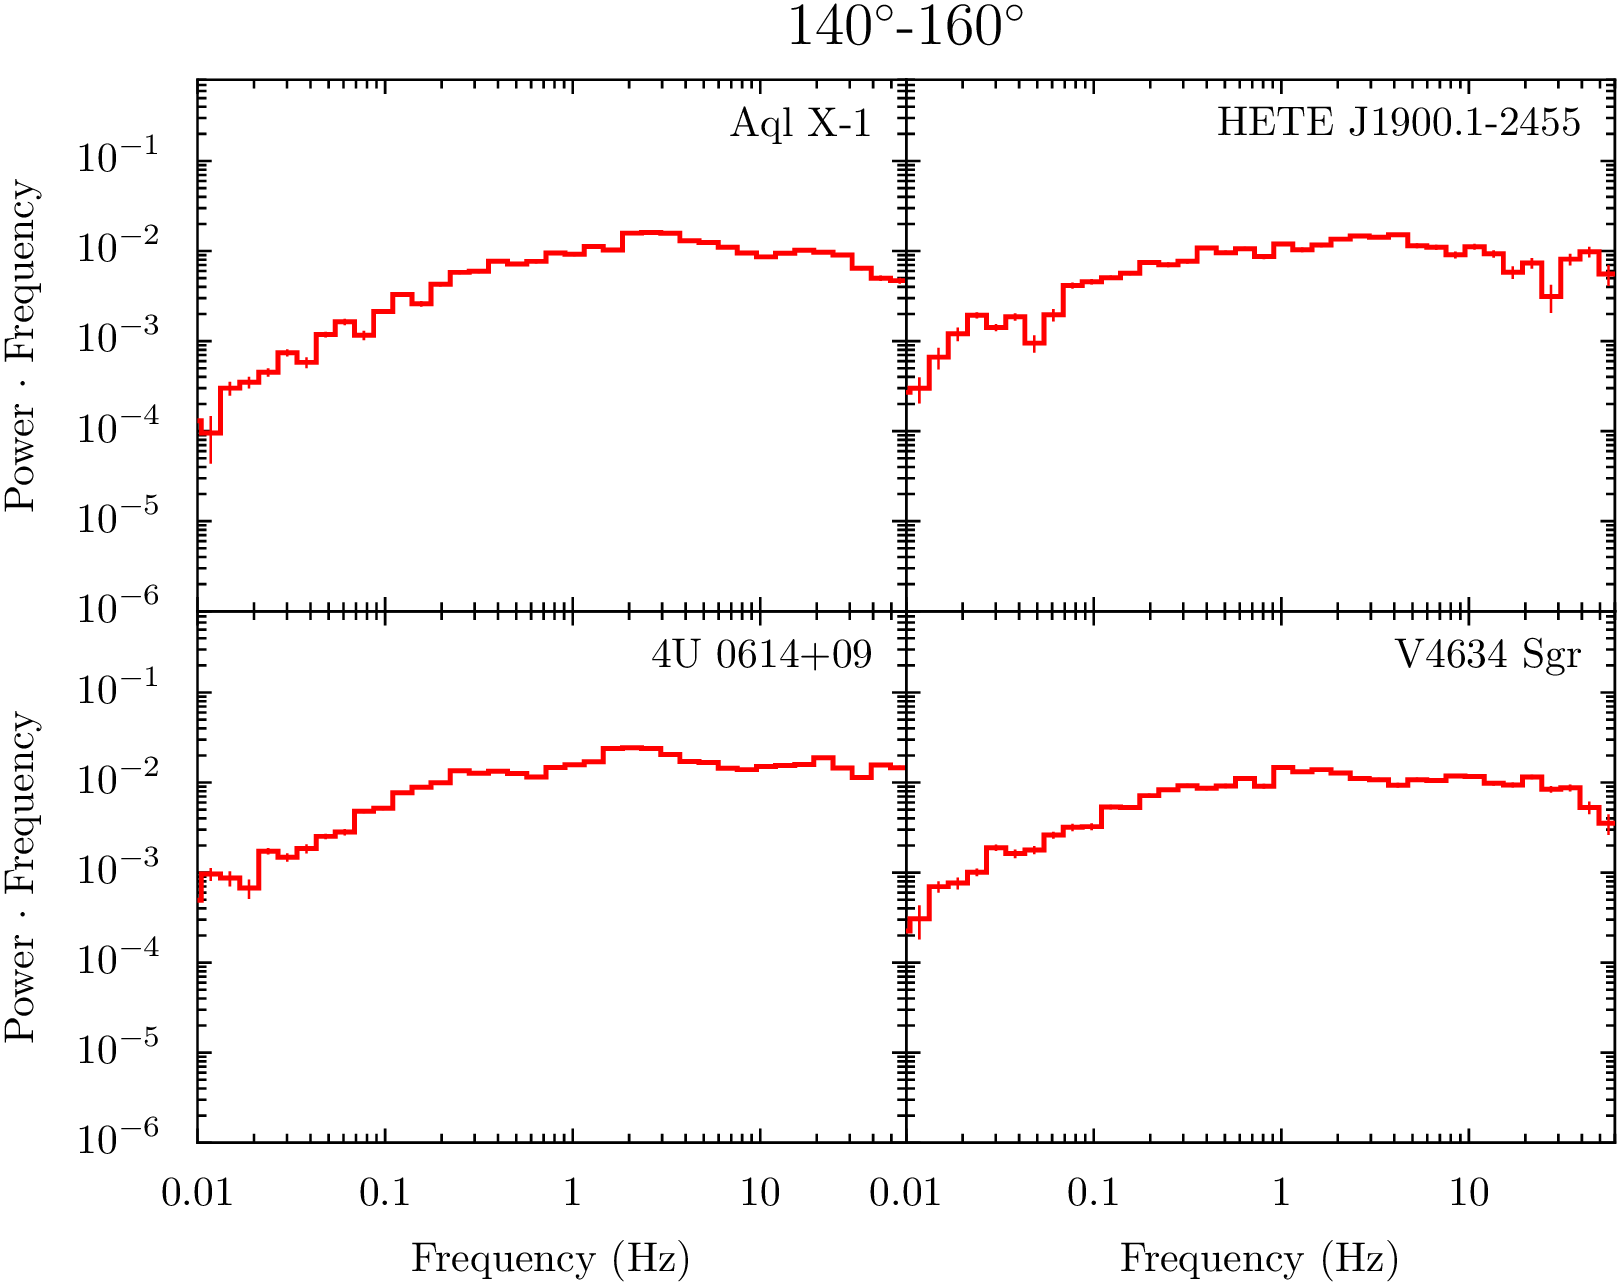
\includegraphics[width=1.13\linewidth]{ps/140_160}}
%	\caption[Power spectra with a hue of 140$^\circ$--160$^\circ$]{Representative power spectra within a hue range of 140$^\circ$--160$^\circ$}\label{fig:ps_140_160}
%\end{figure}
%
%\begin{figure}[p]
%	%\myfloatalign
%	{\vspace*{-0.5cm}\hspace*{-1.5cm}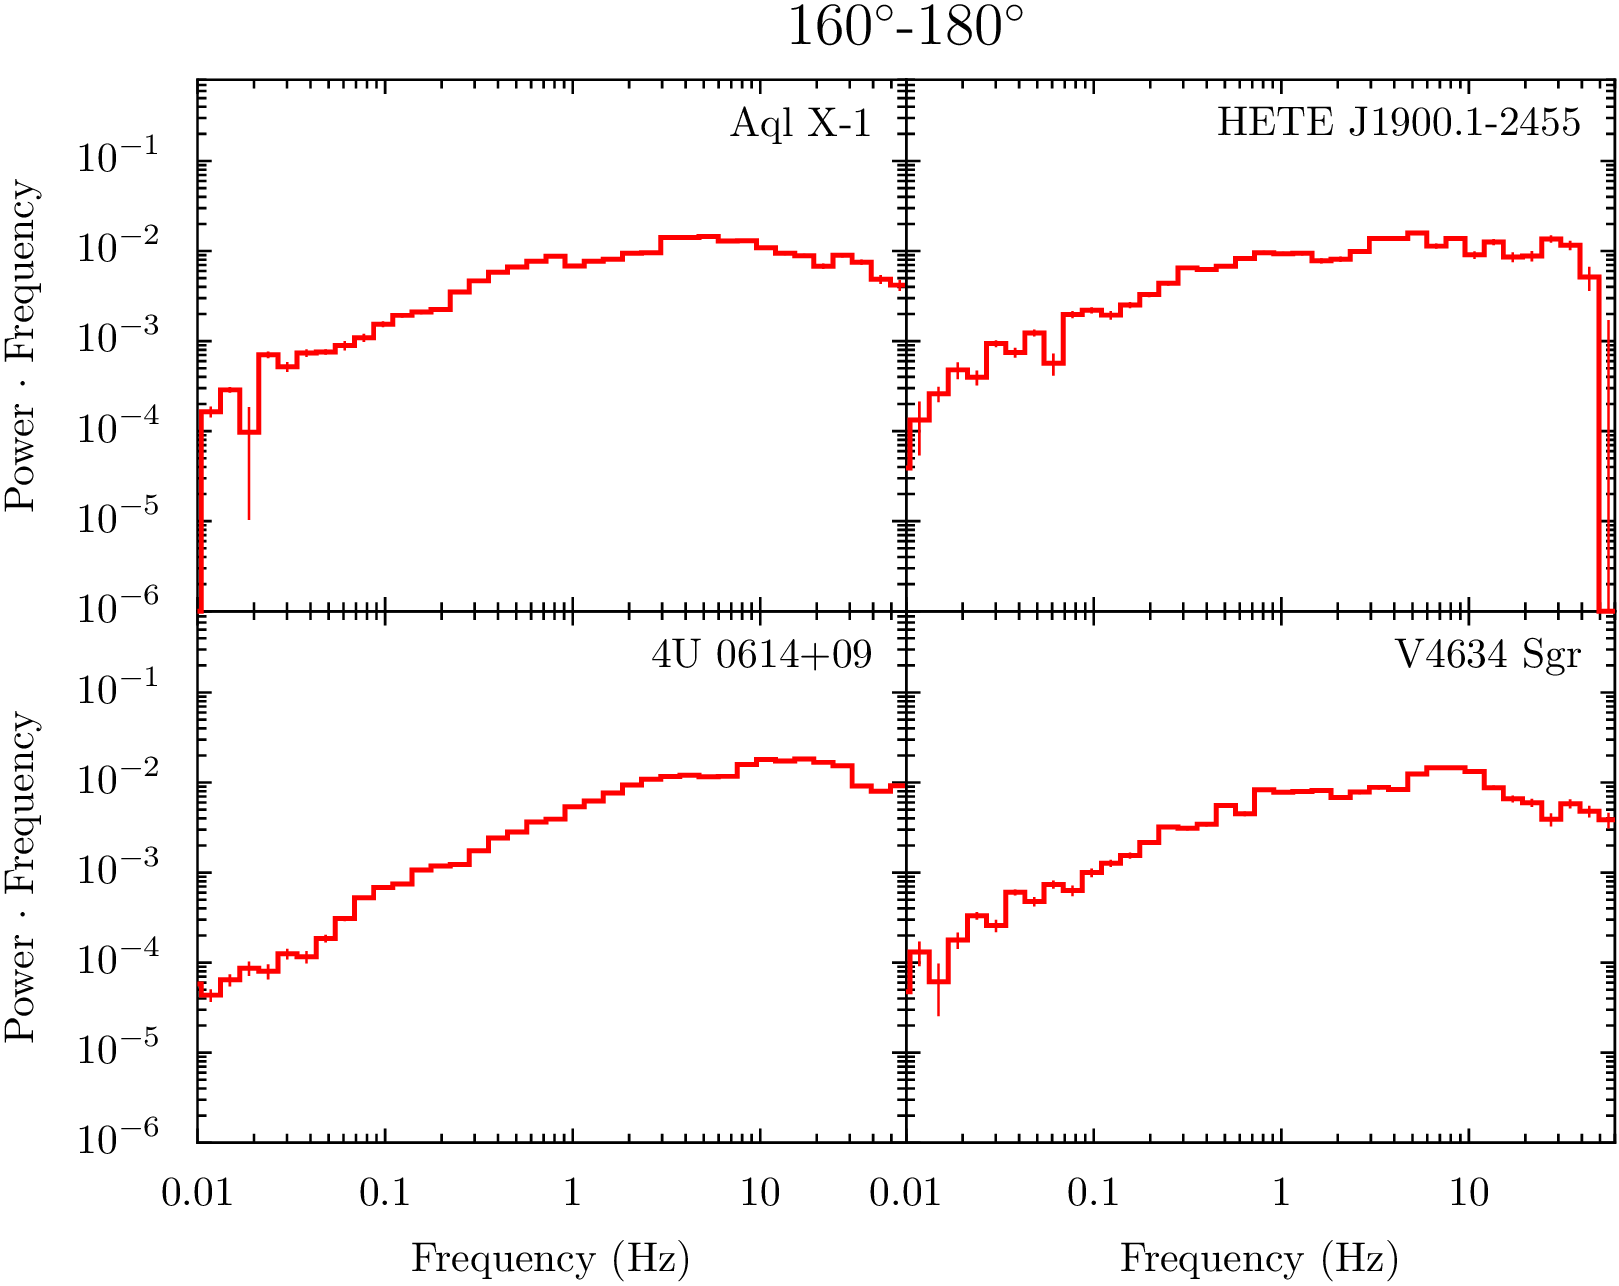
\includegraphics[width=1.13\linewidth]{ps/160_180}}
%	\caption[Power spectra with a hue of 160$^\circ$--180$^\circ$]{Representative power spectra within a hue range of 160$^\circ$--180$^\circ$}\label{fig:ps_160_180}
%\end{figure}
%
%\begin{figure}[p]
%	%\myfloatalign
%	{\vspace*{-0.5cm}\hspace*{-1.5cm}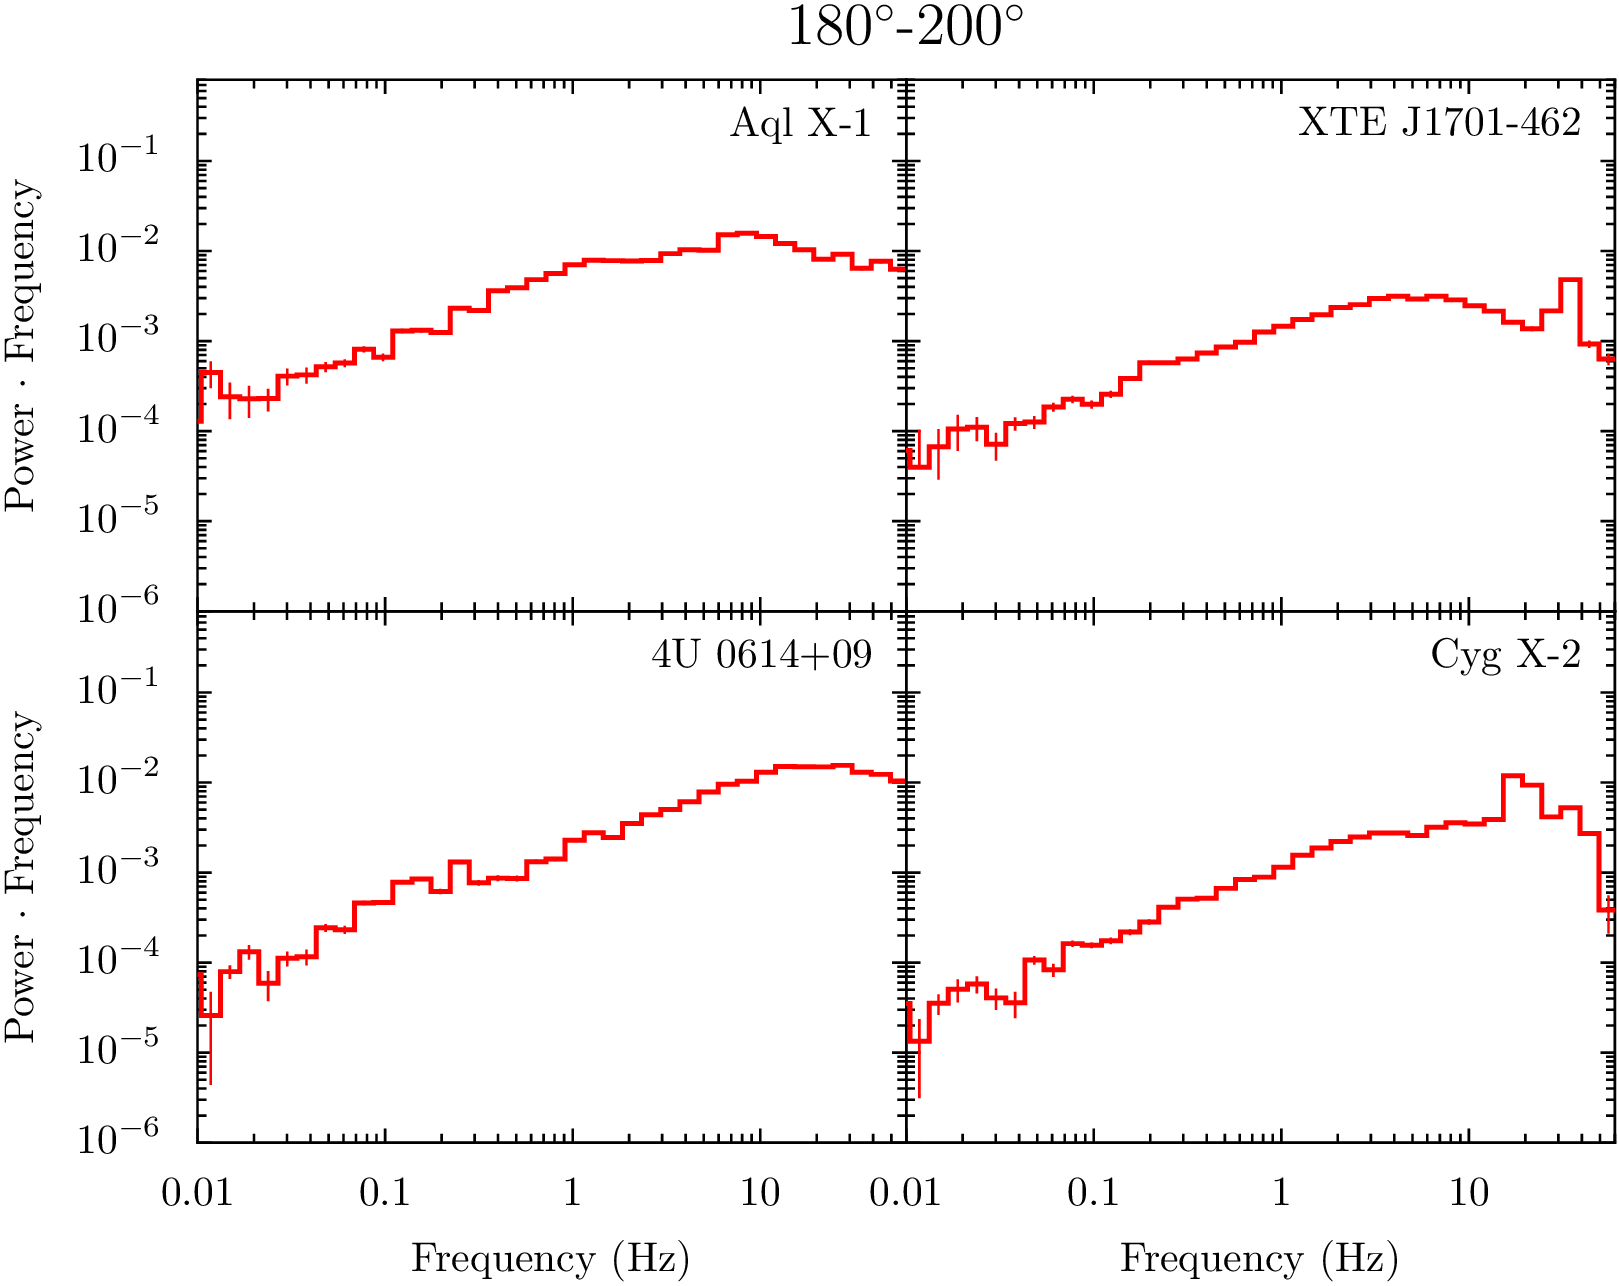
\includegraphics[width=1.13\linewidth]{ps/180_200}}
%	\caption[Power spectra with a hue of 180$^\circ$--200$^\circ$]{Representative power spectra within a hue range of 180$^\circ$--200$^\circ$}\label{fig:ps_180_200}
%\end{figure}
%
%\begin{figure}[p]
%	%\myfloatalign
%	{\vspace*{-0.5cm}\hspace*{-1.5cm}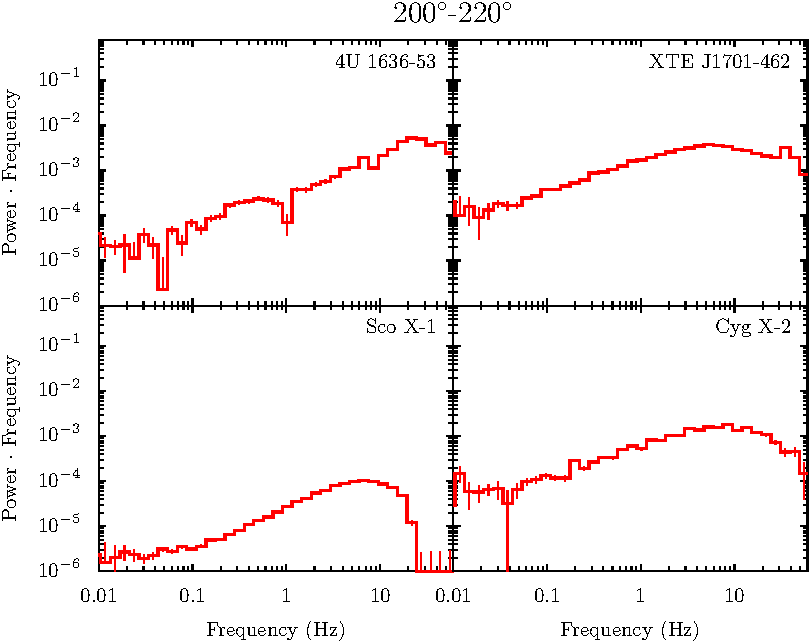
\includegraphics[width=1.13\linewidth]{ps/200_220}}
%	\caption[Power spectra with a hue of 200$^\circ$--220$^\circ$]{Representative power spectra within a hue range of 200$^\circ$--220$^\circ$}\label{fig:ps_200_220}
%\end{figure}
%
%\begin{figure}[p]
%	%\myfloatalign
%	{\vspace*{-0.5cm}\hspace*{-1.5cm}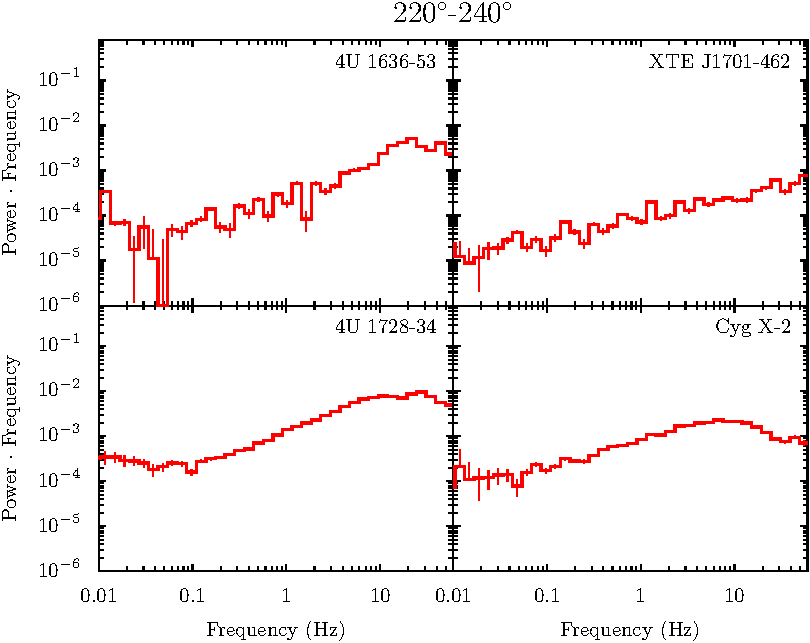
\includegraphics[width=1.13\linewidth]{ps/220_240}}
%	\caption[Power spectra with a hue of 220$^\circ$--240$^\circ$]{Representative power spectra within a hue range of 220$^\circ$--240$^\circ$}\label{fig:ps_220_240}
%\end{figure}
%
%\begin{figure}[p]
%	%\myfloatalign
%	{\vspace*{-0.5cm}\hspace*{-1.5cm}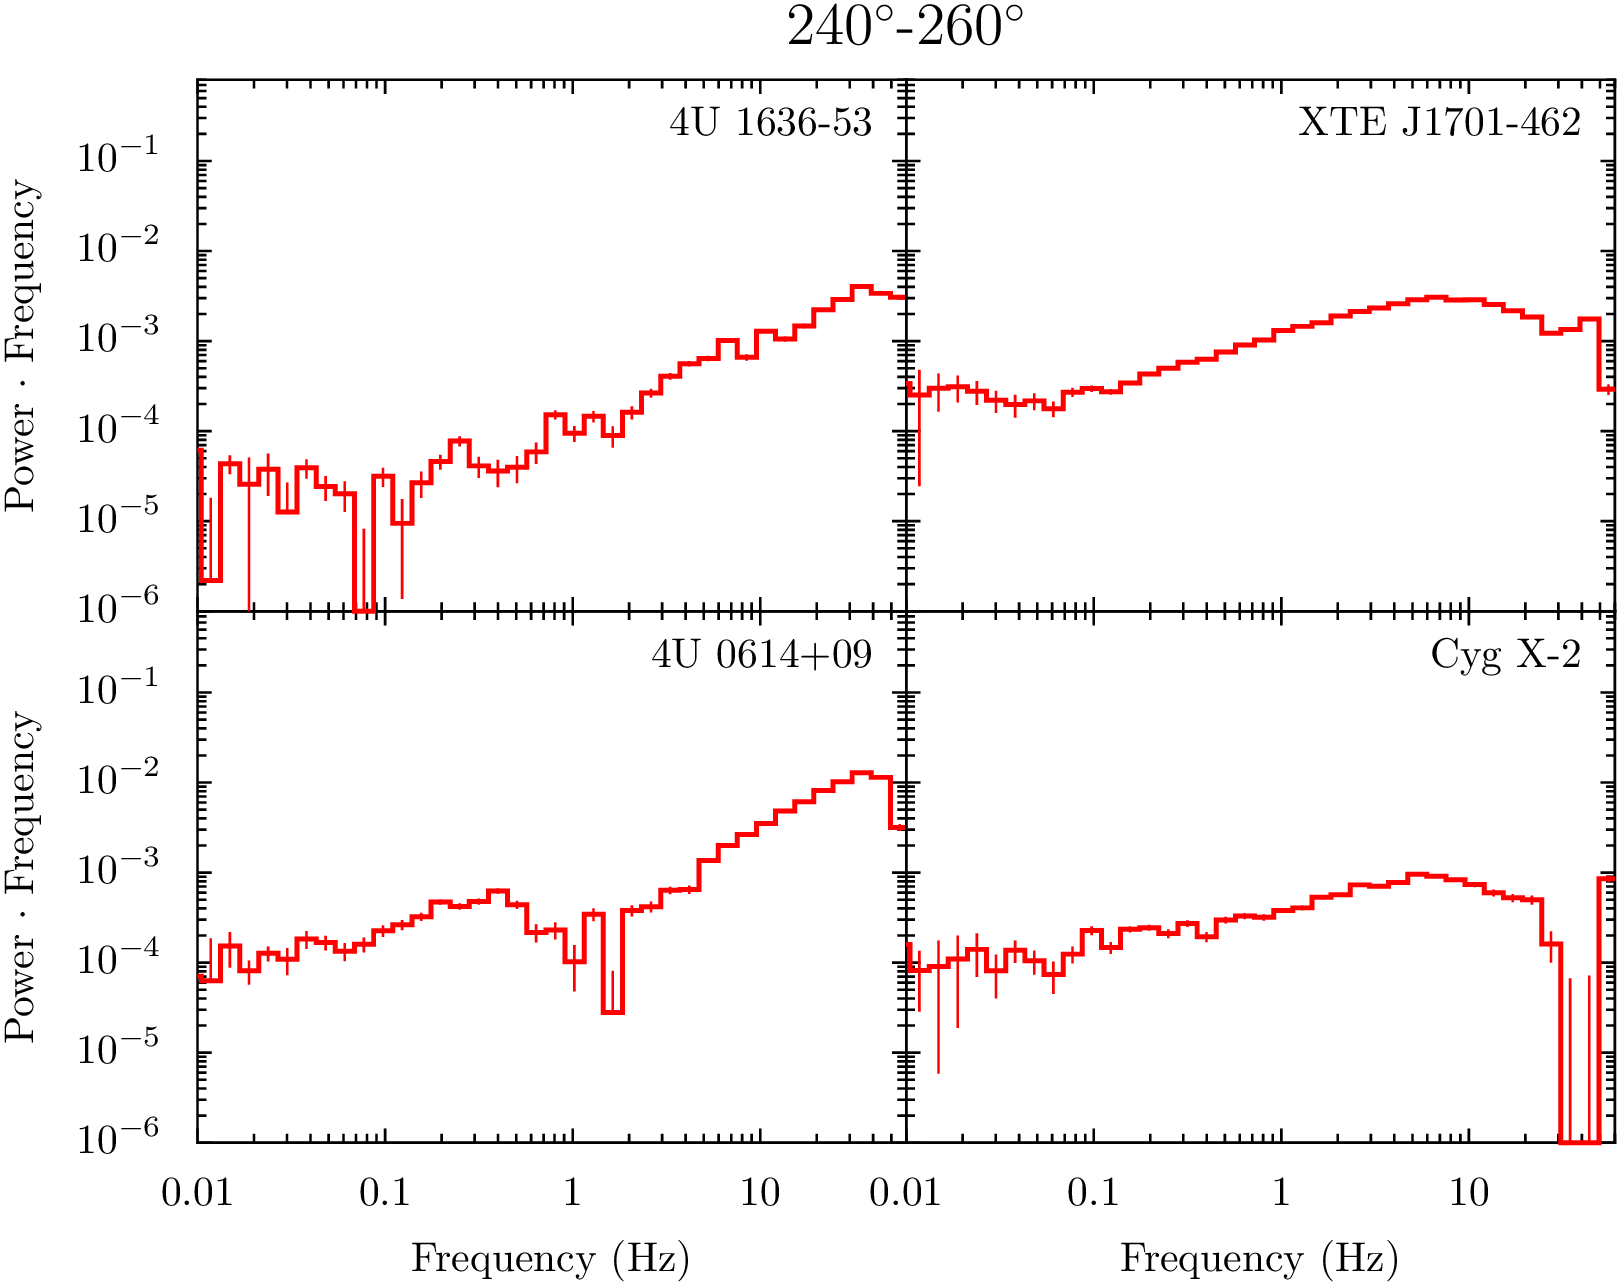
\includegraphics[width=1.13\linewidth]{ps/240_260}}
%	\caption[Power spectra with a hue of 240$^\circ$--260$^\circ$]{Representative power spectra within a hue range of 240$^\circ$--260$^\circ$}\label{fig:ps_240_260}
%\end{figure}
%
%\begin{figure}[p]
%	%\myfloatalign
%	{\vspace*{-0.5cm}\hspace*{-1.5cm}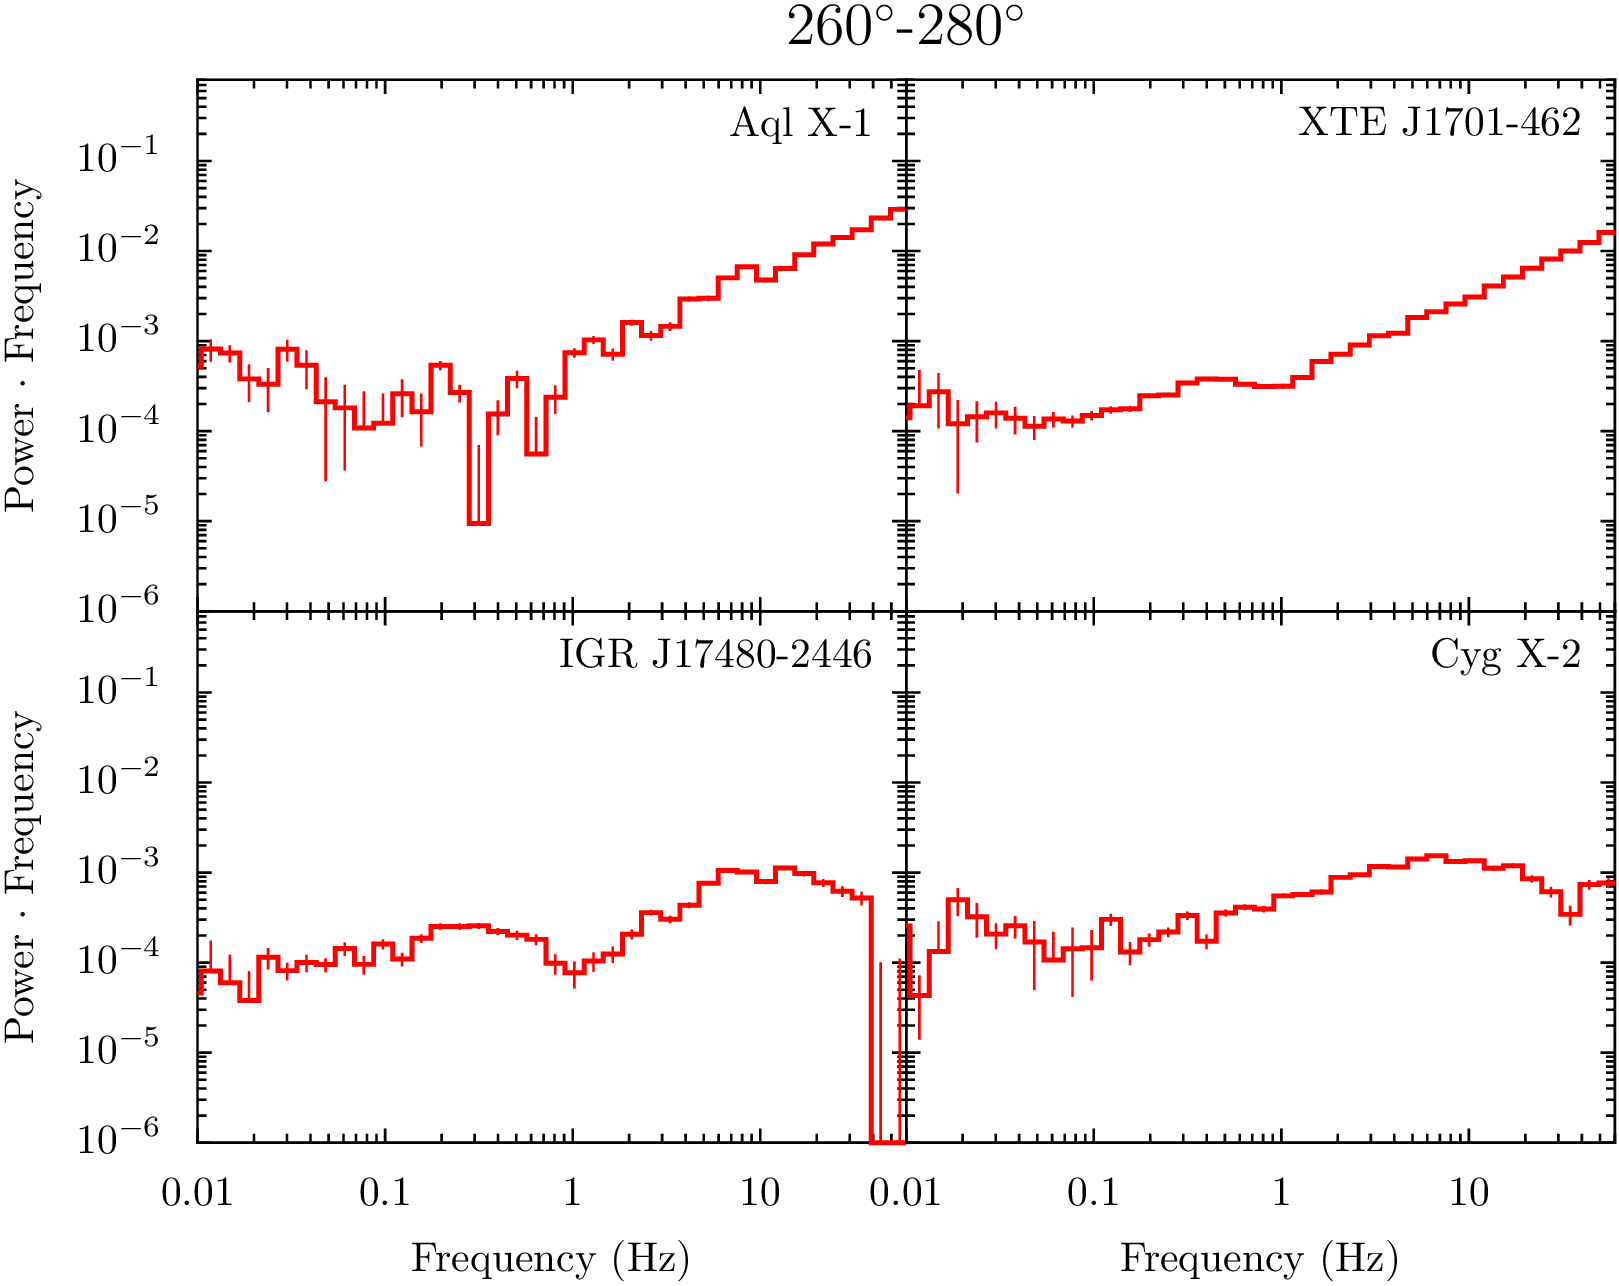
\includegraphics[width=1.13\linewidth]{ps/260_280}}
%	\caption[Power spectra with a hue of 260$^\circ$--280$^\circ$]{Representative power spectra within a hue range of 260$^\circ$--280$^\circ$}\label{fig:ps_260_280}
%\end{figure}
%
%\begin{figure}[p]
%	%\myfloatalign
%	{\vspace*{-0.5cm}\hspace*{-1.5cm}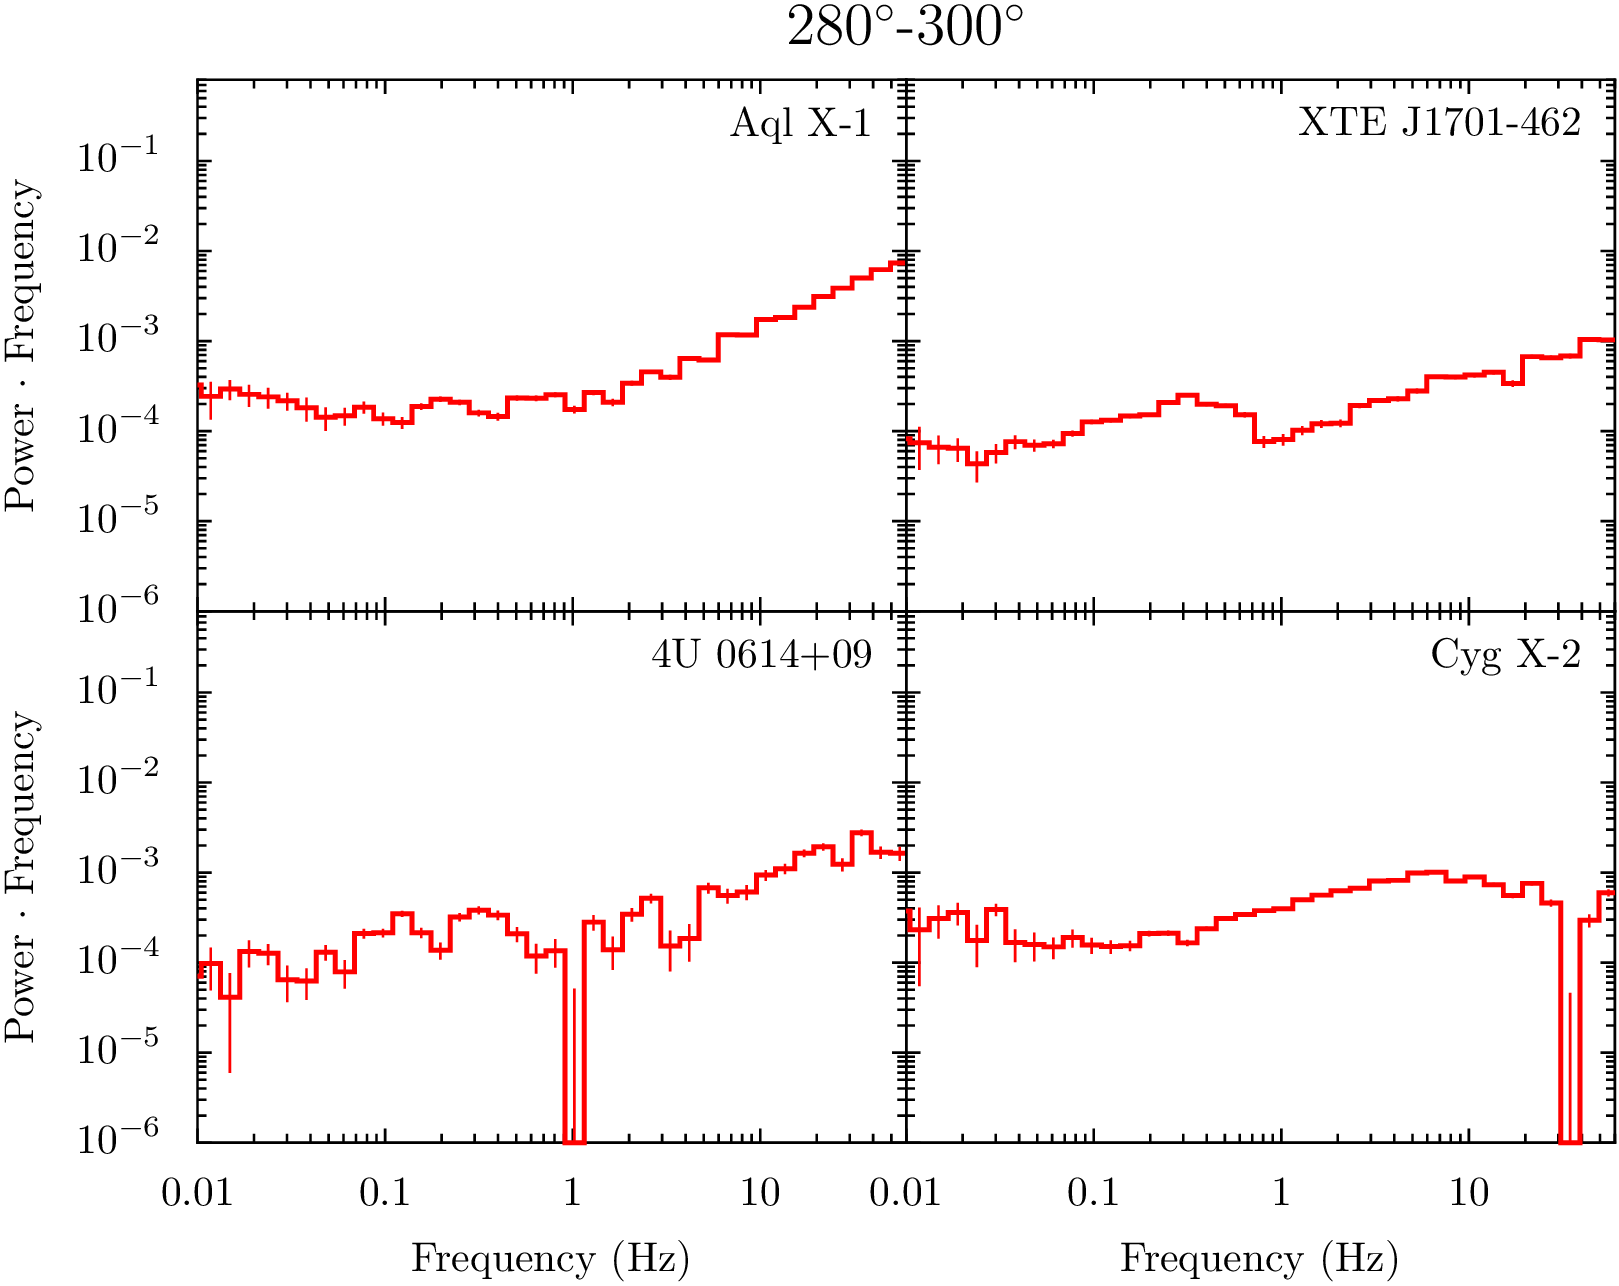
\includegraphics[width=1.13\linewidth]{ps/280_300}}
%	\caption[Power spectra with a hue of 280$^\circ$--300$^\circ$]{Representative power spectra within a hue range of 280$^\circ$--300$^\circ$}\label{fig:ps_280_300}
%\end{figure}
%
%\begin{figure}[p]
%	%\myfloatalign
%	{\vspace*{-0.5cm}\hspace*{-1.5cm}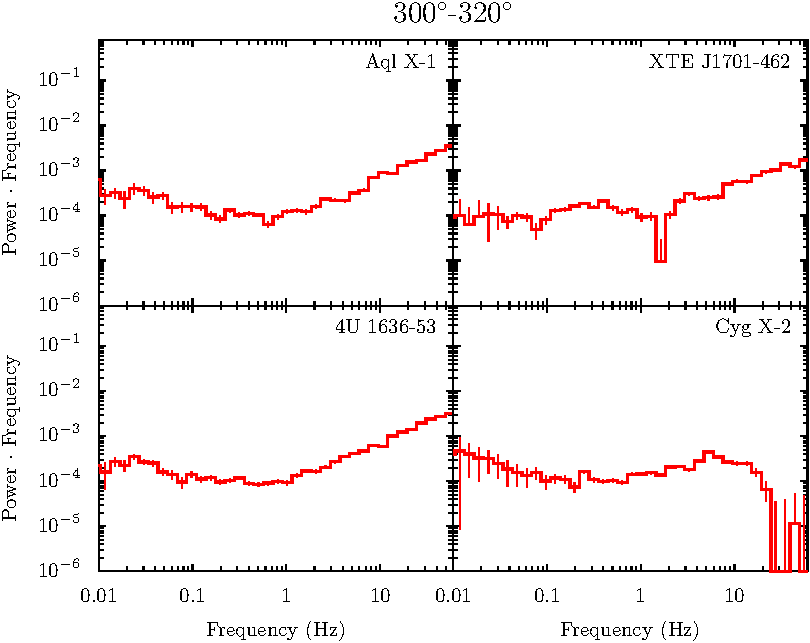
\includegraphics[width=1.13\linewidth]{ps/300_320}}
%	\caption[Power spectra with a hue of 300$^\circ$--320$^\circ$]{Representative power spectra within a hue range of 300$^\circ$--320$^\circ$}\label{fig:ps_300_320}
%\end{figure}
%
%\begin{figure}[p]
%	%\myfloatalign
%	{\vspace*{-0.5cm}\hspace*{-1.5cm}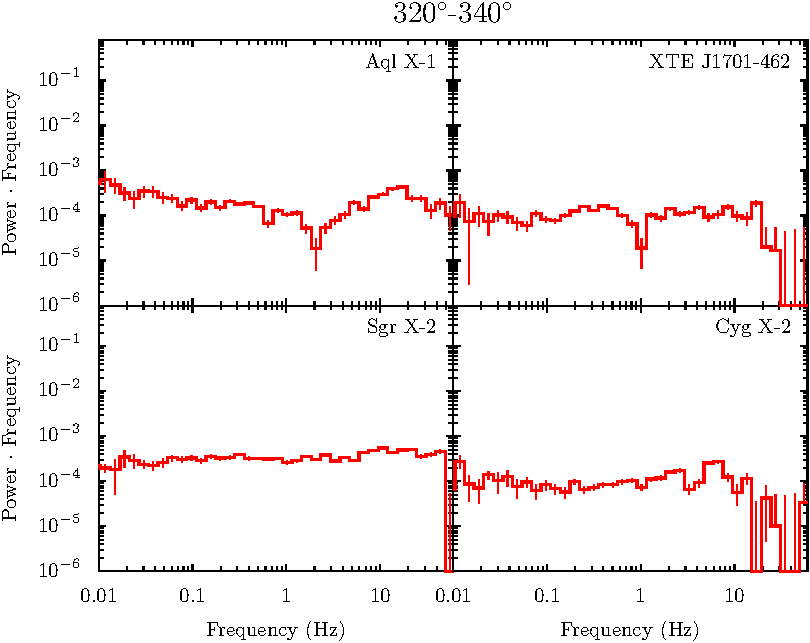
\includegraphics[width=1.13\linewidth]{ps/320_340}}
%	\caption[Power spectra with a hue of 320$^\circ$--340$^\circ$]{Representative power spectra within a hue range of 320$^\circ$--340$^\circ$}\label{fig:ps_320_340}
%\end{figure}
%\begin{figure}[p]
%	%\myfloatalign
%	{\vspace*{-0.5cm}\hspace*{-1.5cm}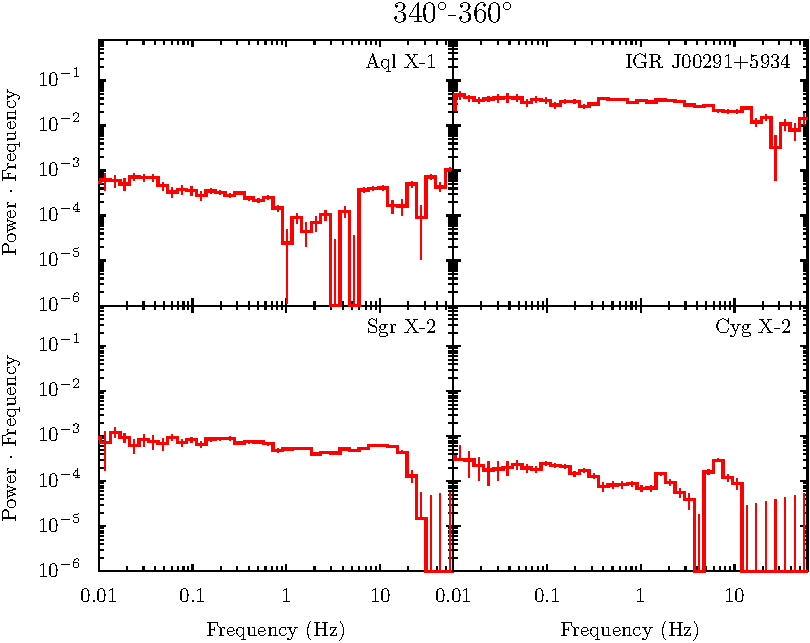
\includegraphics[width=1.13\linewidth]{ps/340_360}}
%	\caption[Power spectra with a hue of 340$^\circ$--360$^\circ$]{Representative power spectra within a hue range of 340$^\circ$--360$^\circ$}\label{fig:ps_340_360}
%\end{figure}
%
%\captionsetup[figure]{list=yes}
%\chapter{Power Colour-Colour Diagrams}
%\label{ch:pccds}
%\begin{figure}[p]
%	%\myfloatalign
%	{\vspace*{-0cm}\hspace*{-3cm}\includegraphics[width=1.45\linewidth]{pc/pane_1}}
%	\caption{\acs{PCC}~diagrams for 4U to GX}\label{fig:pc_pane_1}
%\end{figure}
%\captionsetup[figure]{list=no}
%\begin{figure}[p]
%	%\myfloatalign
%	{\vspace*{-0cm}\hspace*{-3cm}\includegraphics[width=1.45\linewidth]{pc/pane_2}}
%	\caption{\acs{PCC}~diagrams for GX to V4}\label{fig:pc_pane_2}
%\end{figure}
%
%\begin{figure}[p]
%	%\myfloatalign
%	{\vspace*{-0cm}\hspace*{-3cm}\includegraphics[width=1.45\linewidth]{pc/pane_3}}
%	\caption{\acs{PCC}~diagrams for XB to XTE}\label{fig:pc_pane_3}
%\end{figure}
%
%\begin{figure}[p]
%	%\myfloatalign
%	{\vspace*{-0cm}\hspace*{-3cm}\includegraphics[width=1.45\linewidth]{pc/pane_4}}
%	\caption{\acs{PCC}~diagrams for black holes}\label{fig:pc_pane_4}
%\end{figure}
%
%\captionsetup[figure]{list=yes}
%\chapter{Hardness-Hue Diagrams}
%\label{ch:hhds}
%\begin{figure}[p]
%	%\myfloatalign
%	{\vspace*{-0cm}\hspace*{-3cm}\includegraphics[width=1.45\linewidth]{hh/pane_1}}
%	\caption{\acs{HH}~diagrams for 4U to GX}\label{fig:hh_pane_1}
%\end{figure}
%\captionsetup[figure]{list=no}
%\begin{figure}[p]
%	%\myfloatalign
%	{\vspace*{-0cm}\hspace*{-3cm}\includegraphics[width=1.45\linewidth]{hh/pane_2}}
%	\caption{\acs{HH}~diagrams for GX to V4}\label{fig:hh_pane_2}
%\end{figure}
%
%\begin{figure}[p]
%	%\myfloatalign
%	{\vspace*{-0cm}\hspace*{-3cm}\includegraphics[width=1.45\linewidth]{hh/pane_3}}
%	\caption{\acs{HH}~diagrams for XB to XTE}\label{fig:hh_pane_3}
%\end{figure}
%
%\begin{figure}[p]
%	%\myfloatalign
%	{\vspace*{-0cm}\hspace*{-3cm}\includegraphics[width=1.45\linewidth]{hh/pane_4}}
%	\caption{\acs{HH}~diagrams for black holes}\label{fig:hh_pane_4}
%\end{figure}
%
%\captionsetup[figure]{list=yes}
%\chapter{Hardness-Intensity Diagrams}
%\label{ch:hids}
%\begin{figure}[p]
%	%\myfloatalign
%	{\vspace*{-0cm}\hspace*{-3cm}\includegraphics[width=1.45\linewidth]{hi/pane_1}}
%	\caption{\acs{HI}~diagrams for 4U to GX}\label{fig:hi_pane_1}
%\end{figure}
%\captionsetup[figure]{list=no}
%\begin{figure}[p]
%	%\myfloatalign
%	{\vspace*{-0cm}\hspace*{-3cm}\includegraphics[width=1.45\linewidth]{hi/pane_2}}
%	\caption{\acs{HI}~diagrams for GX to V4}\label{fig:hi_pane_2}
%\end{figure}
%
%\begin{figure}[p]
%	%\myfloatalign
%	{\vspace*{-0cm}\hspace*{-3cm}\includegraphics[width=1.45\linewidth]{hi/pane_3}}
%	\caption{\acs{HI}~diagrams for XB to XTE}\label{fig:hi_pane_3}
%\end{figure}
%
%\begin{figure}[p]
%	%\myfloatalign
%	{\vspace*{-0cm}\hspace*{-3cm}\includegraphics[width=1.45\linewidth]{hi/pane_4}}
%	\caption{\acs{HI}~diagrams for black holes}\label{fig:hi_pane_4}
%\end{figure}